\documentclass[xcolor=table]{beamer}
%------------------------------------------------------------
% Theme and Appearance
%------------------------------------------------------------
\usetheme[footline=authorinstitutetitle]{Berlin} 
\setbeamertemplate{navigation symbols}{} 

% Headline with Access Code
\setbeamertemplate{headline}{
    \begin{beamercolorbox}[wd=\paperwidth,ht=2.5ex,dp=1ex,right]{section in head/foot}
        \usebeamerfont{section in head/foot}
        \hspace{0.5cm}
        \ifnum\insertframenumber<30
            \raisebox{-1pt}[0pt][0pt]{\normalsize\textbf{Attendance Code: 510293}}
        \fi
        \hspace{0.5cm}
    \end{beamercolorbox}
}
% Footline with page numbers
\setbeamertemplate{footline}{
    \leavevmode%
    \hbox{%
        \begin{beamercolorbox}[wd=.333333\paperwidth,ht=2.25ex,dp=1ex,left]{author in head/foot}%
            \usebeamerfont{author in head/foot}\hspace*{0.5em}\insertshortauthor
        \end{beamercolorbox}%
        \begin{beamercolorbox}[wd=.333333\paperwidth,ht=2.25ex,dp=1ex,center]{title in head/foot}%
            \usebeamerfont{title in head/foot}\insertshorttitle
        \end{beamercolorbox}%
        \begin{beamercolorbox}[wd=.333333\paperwidth,ht=2.25ex,dp=1ex,right]{date in head/foot}%
            \usebeamerfont{date in head/foot}\insertshortdate{}\hspace*{2em}
            \insertframenumber{} / \inserttotalframenumber\hspace*{2ex} 
        \end{beamercolorbox}}%
    \vskip0pt%
}
\usepackage[utf8]{inputenc}
\usepackage[table]{xcolor}
\usepackage{colortbl}
\usepackage{minted}
\usepackage{lmodern}
\usepackage{tgheros}
\usepackage{hyperref}
\usepackage{tikz}
\usetikzlibrary{shapes, arrows, arrows.meta, positioning, shadows, fit, calc, backgrounds}

\renewcommand*\familydefault{\sfdefault}

% Agenda at the start of every section
\AtBeginSection[]
{
    \begin{frame}
        \frametitle{Agenda}
        \tableofcontents[currentsection]
    \end{frame}
}

%------------------------------------------------------------
% Title Page Information
%------------------------------------------------------------
\title[CMP9134 - Week 12]{Software Evolution \& Technical Debt}
\subtitle{CMP9134: Software Engineering}
\author[Francesco Del Duchetto]{Dr Francesco Del Duchetto\\Lecturer in Robotics and Autonomous Systems}
\institute[University of Lincoln]{University of Lincoln}
\date{24 April 2026}

%------------------------------------------------------------
\begin{document}

%--- TITLE FRAME ---
\begin{frame}
    \titlepage
\end{frame}

%--- AGENDA FRAME ---
\begin{frame}
    \frametitle{Today's Agenda}
    \tableofcontents
\end{frame}

%------------------------------------------------------------
\section{Recap \& Introduction}
%------------------------------------------------------------

\begin{frame}
    \frametitle{The Journey So Far}
    Over the past 11 weeks, we have covered the journey of \textbf{building} software:
    
    \begin{itemize}
        \item \textbf{Weeks 1-3:} Agile Planning, Requirements, and UML Models.
        \item \textbf{Weeks 4-6:} System Architecture, Design Patterns, and HCI.
        \item \textbf{Weeks 7-9:} Containerisation (Docker) and Automated CI/CD Pipelines.
    \end{itemize}
    
    \vspace{0.3cm}
    You have built your Ground Control Station. Your tests are passing. Your containers are running. Is the Software Engineering process over?
    
    \vspace{0.2cm}
    \textbf{No. In fact, it is just beginning.}
\end{frame}

\begin{frame}
    \frametitle{Today's Learning Objectives}
    By the end of this lecture, you should be able to:
    \begin{enumerate}
        \item \textbf{Understand} the principles of Software Evolution and Lehman's Laws.
        \item \textbf{Define} Technical Debt and analyze its impact on software lifecycles.
        \item \textbf{Identify} common "Code Smells" that indicate poor design.
        \item \textbf{Apply} Refactoring techniques to improve code quality without altering external behavior.
    \end{enumerate}
\end{frame}

%------------------------------------------------------------
\section{Software Evolution}
%------------------------------------------------------------

\begin{frame}
    \frametitle{The Reality of Software}
    Software is not a physical bridge. When a bridge is built, it remains static until it decays. Software, however, is a living entity.
    
    \vspace{0.3cm}
    \begin{block}{Software Evolution}
        The process of developing, maintaining, and updating software \textit{after} its initial release to accommodate changing user requirements, hardware updates, or business goals.
    \end{block}
    
    \vspace{0.3cm}
    \textbf{Why does software evolve?}
    \begin{itemize}
        \item The business environment changes (e.g., new robotics regulations).
        \item Underlying platforms change (e.g., Python 2 is deprecated for Python 3).
        \item Users discover new ways to use the system that developers never anticipated.
    \end{itemize}
\end{frame}

\begin{frame}
    \frametitle{Lehman's Laws of Software Evolution}
    In the 1970s, Meir Lehman proposed a set of laws regarding software evolution. They remain universally true today.
    
    \vspace{0.3cm}
    \textbf{1. The Law of Continuing Change:}
    A system must continually adapt to its changing environment, or it will become progressively less useful until it dies.
    
    \vspace{0.2cm}
    \textbf{2. The Law of Increasing Complexity:}
    As a system evolves, its complexity increases unless explicit work is done to maintain or reduce it.
    
    \vspace{0.2cm}
    \textbf{3. The Law of Declining Quality:}
    The quality of a system will appear to decline over time unless it is rigorously maintained and adapted to changes in its operational environment.
\end{frame}

%------------------------------------------------------------
\section{Technical Debt}
%------------------------------------------------------------

\begin{frame}
    \frametitle{What is Technical Debt?}
    As complexity increases (Lehman's 2nd Law), teams often take shortcuts to deliver features faster. This introduces \textbf{Technical Debt}.
    
    \vspace{0.3cm}
    \begin{alertblock}{The Financial Metaphor (Ward Cunningham)}
        Shipping first-time code is like going into debt. A little debt speeds development so long as it is paid back promptly with a rewrite. The danger occurs when the debt is not repaid. Every minute spent on not-quite-right code counts as \textbf{interest} on that debt.
    \end{alertblock}
    
    \vspace{0.2cm}
    \textbf{How do we pay the "interest"?}
    \begin{itemize}
        \item Slower development times for future features.
        \item Increased bug rates.
        \item Developer burnout and frustration.
    \end{itemize}
\end{frame}

\begin{frame}[fragile]
    \frametitle{The Technical Debt Quadrant (Martin Fowler)}
    Not all technical debt is bad. Sometimes it is a strategic business decision.
    
    \vspace{0.3cm}
    \centering
    \resizebox{0.8\textwidth}{!}{
    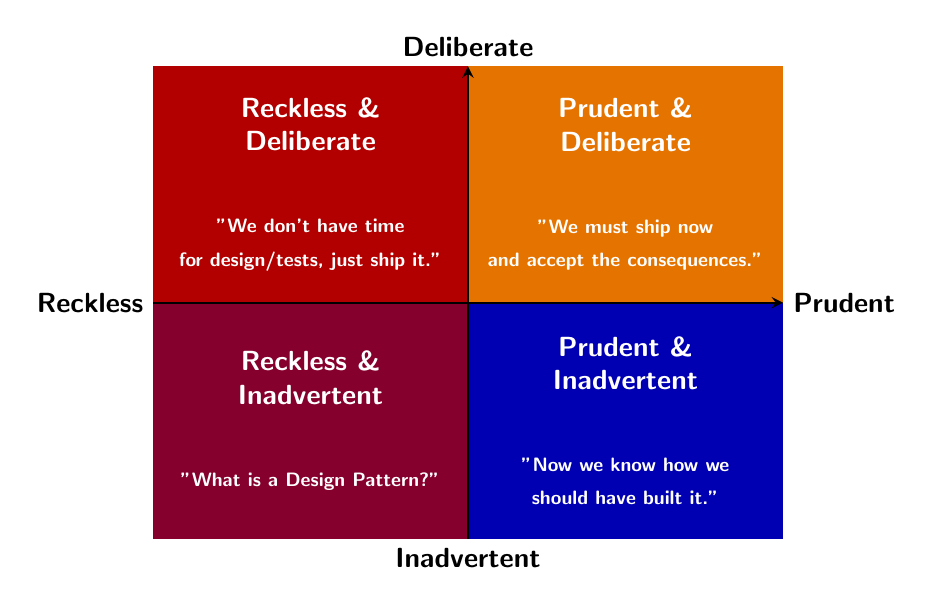
\begin{tikzpicture}[
        quadrant/.style={rectangle, text=white, font=\sffamily\bfseries, align=center, minimum width=4cm, minimum height=3cm},
        axis/.style={thick, -stealth}
    ]
        % Quadrants
        \node[quadrant, fill=red!70!black] (reckless_deliberate) at (-2, 1.5) {Reckless \&\\Deliberate\\ \vspace{0.2cm}\\ \scriptsize "We don't have time\\ \scriptsize for design/tests, just ship it."};
        \node[quadrant, fill=orange!90!black] (prudent_deliberate) at (2, 1.5) {Prudent \&\\Deliberate\\ \vspace{0.2cm}\\ \scriptsize "We must ship now\\ \scriptsize and accept the consequences."};
        \node[quadrant, fill=purple!70!black] (reckless_inadvertent) at (-2, -1.5) {Reckless \&\\Inadvertent\\ \vspace{0.2cm}\\ \scriptsize "What is a Design Pattern?"};
        \node[quadrant, fill=blue!70!black] (prudent_inadvertent) at (2, -1.5) {Prudent \&\\Inadvertent\\ \vspace{0.2cm}\\ \scriptsize "Now we know how we\\ \scriptsize should have built it."};
        
        % Axes
        \draw[axis] (-4, 0) -- (4, 0) node[right, font=\bfseries] {Prudent};
        \node[left, font=\bfseries] at (-4, 0) {Reckless};
        
        \draw[axis] (0, -3) -- (0, 3) node[above, font=\bfseries] {Deliberate};
        \node[below, font=\bfseries] at (0, -3) {Inadvertent};
    \end{tikzpicture}
    }
\end{frame}

\begin{frame}
    \frametitle{Knowledge Check: Classify the Debt}
    \textbf{Scenario:} 
    Your team is building the Ground Control Station. The deadline is tomorrow. You realize your database queries are unoptimized and might slow down if 1,000 robots connect. 
    
    You decide to ship the code as-is to meet the deadline, but you immediately create a Jira ticket to rewrite the queries next sprint.
    
    \vspace{0.3cm}
    \textbf{Question:} Which quadrant of Technical Debt is this?
    \begin{enumerate}
        \item A) Reckless \& Deliberate
        \item B) Prudent \& Inadvertent
        \item C) Prudent \& Deliberate
        \item D) Reckless \& Inadvertent
    \end{enumerate}
    
    \pause
    \vspace{0.3cm}
    \begin{alertblock}{Answer: C (Prudent \& Deliberate)}
        You knew exactly what the consequences were (Deliberate), and you made a calculated business decision while planning for the payback (Prudent).
    \end{alertblock}
\end{frame}
%------------------------------------------------------------
\section{Code Smells}
%------------------------------------------------------------

\begin{frame}
    \frametitle{Identifying Debt: Code Smells}
    How do you know if your codebase has technical debt? You look for \textbf{Code Smells}.
    
    \vspace{0.3cm}
    A code smell is a surface indication that usually corresponds to a deeper problem in the system. It is not necessarily a bug—the code might work perfectly—but it indicates weaknesses in design that increase the risk of future bugs.
\end{frame}

\begin{frame}
    \frametitle{Common Code Smells}
    \begin{itemize}
        \item \textbf{The God Class:} A single class that controls too much, has too many dependencies, and thousands of lines of code. It violates the Single Responsibility Principle.
        \item \textbf{Long Method:} A function that spans multiple screens. It is doing too many things, making it impossible to unit test effectively.
        \item \textbf{Duplicated Code (Copy-Paste Programming):} The same logic exists in three different places. If a bug is found, you have to remember to fix it in all three places.
        \item \textbf{Shotgun Surgery:} Every time you want to make a simple change (e.g., adding a new robot sensor), you have to make tiny edits to 15 different files.
        \item \textbf{Magic Numbers:} Hardcoded numbers scattered through the code (e.g., \texttt{if (status == 4)} instead of \texttt{if (status == ROBOT\_IDLE)}).
    \end{itemize}
\end{frame}

\begin{frame}[fragile]
    \frametitle{Interactive Task: Spot the Smells}
    Take 60 seconds. Read the code below. How many distinct "Code Smells" can you find?
    
    \begin{minted}[bgcolor=lightgray, fontsize=\scriptsize]{python}
def do_stuff(x):
    if x == 1:
        # connect to DB
        db.execute("UPDATE robots SET status = 'active' WHERE id = 1")
    elif x == 2:
        # connect to DB
        db.execute("UPDATE robots SET status = 'active' WHERE id = 2")
    # ... repeats 10 more times ...
    print("Done checking. Now let's calculate battery...")
    # ... 50 more lines of battery calculation logic ...
    \end{minted}
    
    \pause
    \vspace{0.2cm}
    \textbf{The Smells:}
    \begin{itemize}
        \item \textbf{Magic Numbers:} What do \texttt{1} and \texttt{2} mean? (Should be named constants).
        \item \textbf{Duplicated Code:} The DB connection and update logic is copy-pasted.
        \item \textbf{Long Method / God Class:} Doing DB updates AND battery calculations in one function called \texttt{do\_stuff}.
    \end{itemize}
\end{frame}

%------------------------------------------------------------
\section{Refactoring}
%------------------------------------------------------------

\begin{frame}
    \frametitle{The Solution: Refactoring}
    If Technical Debt is the disease, Refactoring is the cure.
    
    \vspace{0.3cm}
    \begin{block}{Refactoring Definition}
        A change made to the internal structure of software to make it easier to understand and cheaper to modify \textbf{without changing its observable behavior}.
    \end{block}
    
    \vspace{0.3cm}
    \textbf{The Golden Rule of Refactoring:}
    You cannot refactor code if you do not have an automated test suite (Week 8)! If you change the internal structure without tests, you are not refactoring; you are just blindly hoping you didn't break anything.
\end{frame}

\begin{frame}[fragile]
    \frametitle{Refactoring Example: Extract Method}
    \textbf{The Smell:} Long Method with unclear logic.
    
    \begin{minted}[bgcolor=red!5, fontsize=\scriptsize]{python}
# BEFORE REFACTORING
def process_robot_telemetry(data):
    # Calculate battery percentage
    voltage = data['voltage']
    percentage = (voltage - 10.5) / (12.6 - 10.5) * 100
    if percentage > 100: percentage = 100
    if percentage < 0: percentage = 0
    
    # Save to database
    db.connect()
    db.execute(f"INSERT INTO telemetry (battery) VALUES ({percentage})")
    db.close()
    \end{minted}
\end{frame}


\begin{frame}[fragile]
    \frametitle{Think-Pair-Share: How do we fix this?}
    \textbf{The Bad Code:}
    \begin{minted}[bgcolor=red!5, fontsize=\scriptsize]{python}
def process_robot_telemetry(data):
    voltage = data['voltage']
    percentage = (voltage - 10.5) / (12.6 - 10.5) * 100
    if percentage > 100: percentage = 100
    if percentage < 0: percentage = 0
    
    db.connect()
    db.execute(f"INSERT INTO telemetry (battery) VALUES ({percentage})")
    db.close()
    \end{minted}
    
    \vspace{0.3cm}
    \textbf{Task (2 minutes):} Turn to the person next to you. If you had to refactor this using the "Extract Method" technique, what would your new function signatures look like?
    
    \pause
    \vspace{0.2cm}
    \textit{(Let's look at the solution on the next slide...)}
\end{frame}

\begin{frame}[fragile]
    \frametitle{Refactoring Example: Extract Method}
    \textbf{The Fix:} Extract the logic into smaller, testable, named methods.
    
    \begin{minted}[bgcolor=green!5, fontsize=\scriptsize]{python}
# AFTER REFACTORING
def process_robot_telemetry(data):
    percentage = calculate_battery_percentage(data['voltage'])
    save_telemetry_to_db(percentage)

def calculate_battery_percentage(voltage):
    percentage = (voltage - 10.5) / (12.6 - 10.5) * 100
    return max(0, min(percentage, 100))

def save_telemetry_to_db(percentage):
    db.connect()
    db.execute("INSERT INTO telemetry (battery) VALUES (?)", (percentage,))
    db.close()
    \end{minted}
    \vspace{0.1cm}
    \textit{Behavior is identical. Readability, security (SQL injection fix), and testability are drastically improved.}
\end{frame}


\begin{frame}
    \frametitle{When should you refactor?}
    You don't need to schedule a "3-month refactoring sprint". Refactoring should be a continuous, daily habit.
    
    \vspace{0.3cm}
    \begin{itemize}
        \item \textbf{The Rule of Three:} The first time you do something, just do it. The second time, wince at the duplication, but do it. The third time you do the same thing, refactor it.
        \item \textbf{When adding a feature:} If the code is too messy to easily add a new feature, refactor the code first to make the addition easy.
        \item \textbf{The Boy Scout Rule:} "Always leave the campground cleaner than you found it." If you open a file to fix a bug and see a poorly named variable, rename it before you commit.
    \end{itemize}
\end{frame}

%------------------------------------------------------------
\section{Next Steps}
%------------------------------------------------------------

\begin{frame}
    \frametitle{This Week's Lab: Paying off your Debt}
    You have been building your Assessment 1 codebase for several weeks now. It is highly likely you have accumulated Technical Debt.
    
    \vspace{0.3cm}
    In the workshop, you will:
    \begin{itemize}
        \item \textbf{Task 1: Static Analysis:} Install and run a static analysis tool (like SonarLint, ESLint, or Pylint) on your repository to automatically detect Code Smells.
        \item \textbf{Task 2: Identification:} Identify at least 3 major instances of Technical Debt in your own code.
        \item \textbf{Task 3: Refactoring:} Apply formal refactoring techniques to clean the code, ensuring your automated CI tests still pass afterward!
    \end{itemize}
\end{frame}

\begin{frame}
    \frametitle{Reading \& Resources}
    \begin{itemize}
        \item \textbf{Recommended Reading:} 
        Sommerville, \textit{Software Engineering 9th Edition}, Chapter 9 (Software Evolution).
        \item \textbf{Refactoring: Improving the Design of Existing Code} by Martin Fowler (The definitive guide to Code Smells and Refactoring techniques).
        \item \textbf{Refactoring.Guru:} An excellent, visual website detailing dozens of specific code smells and how to fix them.
    \end{itemize}
\end{frame}

\begin{frame}
    \frametitle{Q \& A}
    \begin{center}
        \Huge Any Questions?\\\vspace{0.5cm} 
        \normalsize fdelduchetto@lincoln.ac.uk
    \end{center}
\end{frame}

\end{document}